\documentclass{beamer}

% Should be documentclass beamer

\mode<presentation>
{
%  \usetheme[hideothersubsections]{PaloAlto}
  \usetheme{metropolis}
  \setbeamercovered{transparent}
}

\usepackage{amsfonts}
\usepackage{amsmath}
\usepackage{amssymb}
\usepackage{color}
\usepackage{tikz}
\usepackage{pgfplots}
\usepackage{listings}
\usepackage{courier}
%\usepackage[utf8]{inputenc}
%\usepackage[russian]{babel}

\lstset{
  numbers=left,
  basicstyle=\ttfamily\footnotesize,
  numberstyle=\tiny\color{gray},
  stepnumber=1,
  numbersep=10pt,
}

\newcommand{\iu}{\ensuremath{\mathrm{i}}}
\newcommand{\bbR}{\mathbb{R}}
\newcommand{\bbC}{\mathbb{C}}
\newcommand{\calV}{\mathcal{V}}
\newcommand{\calW}{\mathcal{W}}
\newcommand{\macheps}{\epsilon_{\mathrm{mach}}}
\newcommand{\matlab}{\textsc{Matlab}}

\newcommand{\ddiag}{\operatorname{diag}}
\newcommand{\fl}{\operatorname{fl}}
\newcommand{\nnz}{\operatorname{nnz}}
\newcommand{\tr}{\operatorname{tr}}
\renewcommand{\vec}{\operatorname{vec}}

\newcommand{\vertiii}[1]{{\left\vert\kern-0.25ex\left\vert\kern-0.25ex\left\vert #1
    \right\vert\kern-0.25ex\right\vert\kern-0.25ex\right\vert}}
\newcommand{\ip}[2]{\langle #1, #2 \rangle}
\newcommand{\ipx}[2]{\left\langle #1, #2 \right\rangle}
\newcommand{\order}[1]{O( #1 )}

\newcommand{\kron}{\otimes}


\newcommand{\hdr}[2]{
  \title[CS 5220, Fall 2017]{CS 5220: #2}
  \author{David Bindel}
  \date{#1}
}

\hdr{2017-08-22}{Introduction}

\begin{document}


\begin{frame}
  \titlepage
\end{frame}


\begin{frame}
  \frametitle{CS 5220: Applications of Parallel Computers}

  \begin{center}
    {\small \url{http://www.cs.cornell.edu/courses/cs5220/2017fa/}} \\[1cm]
    \begin{tabular}{ll}
      Time:       & TR 8:40--9:55 \\
      Location:   & Gates G01 \\
      Instructor: & David Bindel ({\tt bindel@cs}) \\
      TA:         & Eric Hans Lee ({\tt erichanslee@cs})
    \end{tabular}
  \end{center}
  
\end{frame}


\begin{frame}
  \frametitle{Enrollment}

  \begin{center}
    {\small \url{http://www.cs.cornell.edu/courseinfo/enrollment}}
  \end{center}

  \begin{itemize}
    \item Many CS classes (including 5220) limit pre-enrollment to
      ensure majors and MEng students can get in.
    \item We almost surely will have enough space for all comers.
    \item Enroll if you want access to class resources.
    \item Enrolling as an auditor is OK.
    \item If you will not take the class, please formally drop!
  \end{itemize}
\end{frame}


\begin{frame}
  \frametitle{The Computational Science \& Engineering Picture}

  \begin{center}
  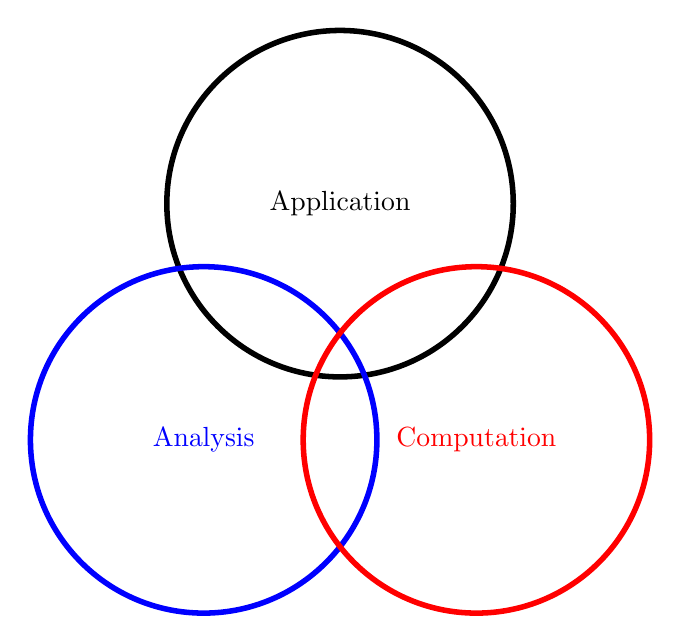
\begin{tikzpicture}
  \draw[black,line width=2pt] (0,2cm) 
    node {Application} circle (2.2 cm);
  \draw[blue,line width=2pt]  (-1.732cm,-1cm) 
    node {Analysis} circle (2.2 cm);
  \draw[red,line width=2pt] ( 1.732cm,-1cm) 
    node {Computation} circle (2.2 cm);
  \end{tikzpicture}
  \end{center}
\end{frame}

\begin{frame}
  \frametitle{Applications Everywhere!}

  These tools are used in more places than you might think:
  \begin{itemize}
  \item Climate modeling
  \item CAD tools (computers, buildings, airplanes, ...)
  \item Control systems
  \item Computational biology
  \item Computational finance
  \item Machine learning and statistical models
  \item Game physics and movie special effects
  \item Medical imaging
  \item Information retrieval
  \item ...
  \end{itemize}
  Parallel computing shows up in all of these.

\end{frame}


\begin{frame}
  \frametitle{Why Parallel Computing?}

  \begin{itemize}
  \item Scientific computing went parallel long ago
    \begin{itemize}
    \item Want an answer that is right enough, fast enough
    \item Either of those might imply a lot of work!
    \item ... and we like to ask for more as machines get bigger
    \item ... and we have a lot of data, too
    \end{itemize}
  \item Today: Hard to get a non-parallel computer!
    \begin{itemize}
    \item Totient nodes (2015): 12-core compute nodes
    \item Totient accelerators (2015): 60-core Xeon Phi 5110P
    \item My laptop (late 2013): Dual core i5 + built in graphics
    \end{itemize}
  \item Cluster access $\approx$ internet connection + credit card
  \end{itemize}
\end{frame}


\begin{frame}
  \frametitle{Lecture Plan}

  Roughly three parts:
  \begin{enumerate}
  \item {\bf Basics:} architecture, parallel concepts, 
    locality and parallelism in scientific codes
  \item {\bf Technology:} OpenMP, MPI, CUDA/OpenCL, cloud systems,
    compilers and tools
  \item {\bf Patterns:} Monte Carlo, dense and sparse linear algebra and PDEs,
    graph partitioning and load balancing, fast multipole, fast transforms
  \end{enumerate}
\end{frame}


\begin{frame}
  \frametitle{Objectives}

  \begin{itemize}
  \item Reason about code performance
    \begin{itemize}
    \item Many factors: HW, SW, algorithms
    \item Want simple ``good enough'' models
    \end{itemize}
  \item Learn about high-performance computing (HPC)
    \begin{itemize}
    \item Learn parallel concepts and vocabulary
    \item Experience parallel platforms (HW and SW)
    \item Read/judge HPC literature
    \item Apply model numerical HPC patterns
    \item Tune existing codes for modern HW
    \end{itemize}
  \item Apply good software practices
  \end{itemize}
\end{frame}


\begin{frame}
  \frametitle{Prerequisites}

  Basic logistical constraints:
  \begin{itemize}
  \item Default class codes will be in C
  \item Our focus is numerical codes
  \end{itemize}

  Fine if you're not a numerical C hacker!
  \begin{itemize}
  \item I want a diverse class
  \item Most students have {\em some} holes
  \item Come see us if you have concerns
  \end{itemize}
\end{frame}


\begin{frame}
  \frametitle{Coursework: Lecture (10\%)}

  \begin{itemize}
  \item Lecture = theory + practical demos
    \begin{itemize}
    \item 60 minutes lecture
    \item 15 minutes mini-practicum
    \item Bring questions for both!
    \end{itemize}
  \item Notes posted in advance
  \item May be prep work for mini-practicum
  \item Course evaluations are also required!
  \end{itemize}
\end{frame}


\begin{frame}
  \frametitle{Coursework: Homework (15\%)}

  \begin{itemize}
  \item Five individual assignments plus ``HW0''
  \item Intent: Get everyone up to speed
  \item Assigned Tues, due one week later
  \end{itemize}
\end{frame}


\begin{frame}
  \frametitle{Coursework: Small group assignments (45\%)}

  \begin{itemize}
  \item Three projects done with partners (1--3)
  \item Analyze, tune, and parallelize a baseline code
  \item Scope is 2-3 weeks
  \end{itemize}
\end{frame}


\begin{frame}
  \frametitle{Coursework: Final project (30\%)}

  \begin{itemize}
  \item Groups are encouraged!
  \item Bring your own topic or we will suggest
  \item Flexible, but {\em must} involve performance
  \item Main part of work in November--December
  \end{itemize}
\end{frame}


\begin{frame}
  \frametitle{Homework 0}

  \begin{itemize}
  \item Posted on the class web page.
  \item Complete and submit by CMS by 8/29.
  \end{itemize}
  
\end{frame}


\begin{frame}
  \begin{center}
    {\large Questions?}
  \end{center}
\end{frame}


\begin{frame}
  \frametitle{How Fast Can We Go?}
  
  Speed records for the Linpack benchmark:
  \begin{center}
  {\small \url{http://www.top500.org}}
  \end{center}

  \vspace{1cm}
  Speed measured in flop/s (floating point ops / second):
  \begin{itemize}
  \item Giga ($10^9$) -- a single core
  \item Tera ($10^{12}$) -- a big machine
  \item Peta ($10^{15}$) -- current top 10 machines (5 in US)
  \item Exa ($10^{18}$) -- favorite of funding agencies
  \end{itemize}

\end{frame}


\begin{frame}
  \frametitle{Current Record: China's Sunway TaihuLight}
  
  \begin{itemize}
  \item 93 petaflop/s (125 petaflop/s peak)
  \item 15 MW (LAPACK) -- relatively energy efficient
    \begin{itemize}
    \item Does not include custom chilled-water cooling unit
    \end{itemize}
  \item Based on SW26010 manycore RISC processors
    \begin{itemize}
    \item Management processing element (CPE) = 64-bit RISC core
    \item Computer processing element (CPE) = $8 \times 8$ core mesh
    \item Custom interconnect
    \item Sunway Raise OS (Linux)
    \item Custom compilers (Sunway OpenACC)
    \end{itemize}
  \end{itemize}
\end{frame}


\begin{frame}
  \frametitle{Performance on TaihuLight (Dongarra, June 2016)}

  \begin{itemize}
  \item Theoretical peak: 125.4 petaflop/s
  \item Linpack: 93 petaflop/s (74\% peak)
  \item Three SC16 Gordon Bell finalists
    \begin{itemize}
    \item Explicit PDE solves: 30--40 petaflop/s (25--30\%)
    \item Implicit solver: 1.5 petaflop/s (1\%)
    \item Numbers taken from June 2016, may have improved
    \item Even with improvements: peak is not indicative!
    \end{itemize}
  \end{itemize}
  
\end{frame}


\begin{frame}
  \frametitle{Second: Tianhe-2 (33.9 pflop/s Linpack)}

  Commodity nodes, custom interconnect:
  \begin{itemize}
  \item
    Nodes consist of Xeon E5-2692 + Xeon Phi accelerators
  \item
    Intel compilers + Intel math kernel libraries
  \item
    MPICH2 MPI with customized channel
  \item
    Kylin Linux
  \item
    \textcolor{red}{\bf TH Express-2}
  \end{itemize}
\end{frame}


\begin{frame}
  \frametitle{Alternate Benchmark: Graph 500}

  Graph processing benchmark (data-intensive)
  \begin{itemize}
  \item Metric: traversed edges per second (TEPS)
  \item K computer (Japan) tops the list (38.6 teraTEPS)
  \item Sunway TaihuLight is second (23.8 teraTEPS)
  \item Tianhe-2 is at 8 (2.1 teraTEPS)
  \end{itemize}
  
\end{frame}


\begin{frame}
  \frametitle{Punchline}

  \begin{itemize}
  \item Some high-end machines look like high-end clusters
    \begin{itemize}
    \item Except custom networks.
    \end{itemize}
  \item Achievable performance is
    \begin{itemize}
    \item $\ll$ peak performance
    \item Application-dependent
    \end{itemize}
  \item Hard to achieve peak on more modest platforms, too!
  \end{itemize}
\end{frame}


\begin{frame}
  \frametitle{Parallel Performance in Practice}

  So how fast can I make my computation?
  \begin{itemize}
  \item Peak $ > $ Linpack $ > $ Gordon Bell $ > $ Typical
  \item Measuring performance of real applications is hard
    \begin{itemize}
    \item Even figure of merit may be unclear (flops, TEPS, ...?)
    \item Typically a few bottlenecks slow things down
    \item And figuring out why they slow down can be tricky!
    \end{itemize}
  \item And we {\em really} care about time-to-solution
    \begin{itemize}
    \item Sophisticated methods get answer in fewer flops
    \item ... but may look bad in benchmarks (lower flop rates!)
    \end{itemize}
  \end{itemize}

  \vspace{7mm}
  See also David Bailey's comments:
  \begin{itemize}
  \item \href{http://crd.lbl.gov/~dhbailey/dhbpapers/twelve-ways.pdf}{\small Twelve Ways to Fool the Masses When Giving Performance Results on Parallel Computers} (1991)
  \item \href{http://crd.lbl.gov/~dhbailey/dhbtalks/dhb-12ways.pdf}{\small Twelve Ways to Fool the Masses: Fast Forward to 2011} (2011)
  \end{itemize}
\end{frame}


\begin{frame}
  \frametitle{Quantifying Parallel Performance}
  
  \begin{itemize}
  \item Starting point: good {\em serial} performance
  \item Strong scaling: compare parallel to serial time on the same
    problem instance as a function of number of processors ($p$)
    \begin{align*}
      \mbox{Speedup} &= \frac{\mbox{Serial time}}{\mbox{Parallel time}} \\[2mm]
      \mbox{Efficiency} &= \frac{\mbox{Speedup}}{p}
    \end{align*}
  \item
    Ideally, speedup = $p$.  
    Usually, speedup $ < p$.
  \item Barriers to perfect speedup
    \begin{itemize}
    \item Serial work (Amdahl's law)
    \item Parallel overheads (communication, synchronization)
    \end{itemize}
  \end{itemize}
\end{frame}


\begin{frame}
  \frametitle{Amdahl's Law}

  Parallel scaling study where some serial code remains:
  \begin{align*}
    p = & \mbox{ number of processors} \\
    s = & \mbox{ fraction of work that is serial} \\
    t_s = & \mbox{ serial time} \\
    t_p = & \mbox{ parallel time} \geq s t_s + (1-s) t_s / p
  \end{align*}

  \vspace{2mm}
  Amdahl's law:
  \[
    \mbox{Speedup} = 
      \frac{t_s}{t_p} = \frac{1}{s + (1-s) / p} > \frac{1}{s}
  \]

  \vspace{5mm}
  So $1\%$ serial work $\implies$ max speedup < $100 \times$,
  regardless of $p$.
\end{frame}


\begin{frame}
  \frametitle{A Little Experiment}
  
  Let's try a simple parallel attendance count:
  \begin{itemize}
  \item {\bf Parallel computation:} Rightmost person in each row 
    counts number in row.
  \item {\bf Synchronization:} Raise your hand when you have a count
  \item {\bf Communication:} When all hands are raised, each row 
        representative adds their count to a tally and says the sum
        (going front to back).
  \end{itemize}

  \vspace{5mm}
  (Somebody please time this.)

\end{frame}


\begin{frame}
  \frametitle{A Toy Analysis}

  Parameters:
  \begin{align*}
    n = & \mbox{ number of students} \\
    r = & \mbox{ number of rows} \\
    t_c = & \mbox{ time to count one student} \\
    t_t = & \mbox{ time to say tally} \\
    t_s \approx & ~n t_c \\
    t_p \approx & ~n t_c / r + r t_t
  \end{align*}

  \vspace{5mm}
  How much could I possibly speed up?

\end{frame}


\begin{frame}
\frametitle{Modeling Speedup}

\begin{center}
  \begin{tikzpicture}
  \begin{axis}[
    width = {\textwidth},
    height = {0.6\textheight},
    xlabel = {Rows},
    ylabel = {Predicted speedup}]
  \addplot file {figs/headcount.dat};
  \end{axis}
  \end{tikzpicture} \\[1cm]
(Parameters: $n = 80$, $t_c = 0.3$, $t_t = 1$.)
\end{center}
\end{frame}


\begin{frame}
\frametitle{Modeling Speedup}

The bound
\[
  \mathrm{speedup} < 
  \frac{1}{2} \sqrt{\frac{n t_c}{t_t}} 
\]
is usually tight.
\vspace{5mm}

Poor speed-up occurs because:
\begin{itemize}
\item The problem size $n$ is small
\item The communication cost is relatively large
\item The serial computation cost is relatively large
\end{itemize}
Some of the usual suspects for parallel performance problems! \\[5mm]
Things would look better if I allowed both $n$ and $r$ to grow ---
that would be a {\em weak} scaling study.

\end{frame}

\begin{frame}
  \frametitle{Summary: Thinking about Parallel Performance}

  Today:
  \begin{itemize}
  \item We're approaching machines with peak {\em exaflop} rates
  \item But codes rarely get peak performance
  \item Better comparison: tuned serial performance
  \item Common measures: {\em speedup} and {\em efficiency}
  \item Strong scaling: study speedup with increasing $p$
  \item Weak scaling: increase both $p$ and $n$
  \item Serial overheads and communication costs kill speedup
  \item Simple analytical models help us understand scaling
  \end{itemize}
\end{frame}

\begin{frame}
  \frametitle{And in case you arrived late}

  \begin{center}
    {\small \url{http://www.cs.cornell.edu/courses/cs5220/2017fa/}}

    \vspace{1cm}
      ... and please enroll and submit HW0!
  \end{center}
  
\end{frame}

\end{document}
